  \subsection{Análisis de la distorsión armónica producida por un amplificador}
    Se propone analizar el siguiente circuito.

      \begin{figure}[H]
        \centering
          \frame{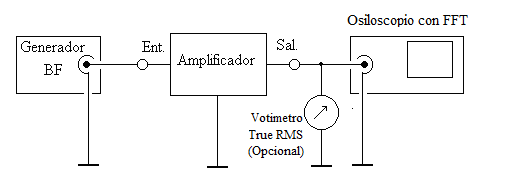
\includegraphics[width=0.8\textwidth]{Imagenes/ActividadPractica/7AnalisisDeDistorisonArmonicaEnAmpli/EsquemaConexionAmplificador.png}}
          \caption{Esquema de circuito a implementar.}
          \label{fig:Exp7EsquemaCircuito}
      \end{figure}

    Se utiliza la placa que se presenta a continuación.

      \begin{figure}[H]
        \centering
        \begin{subfigure}[H]{0.48\textwidth}
          \frame{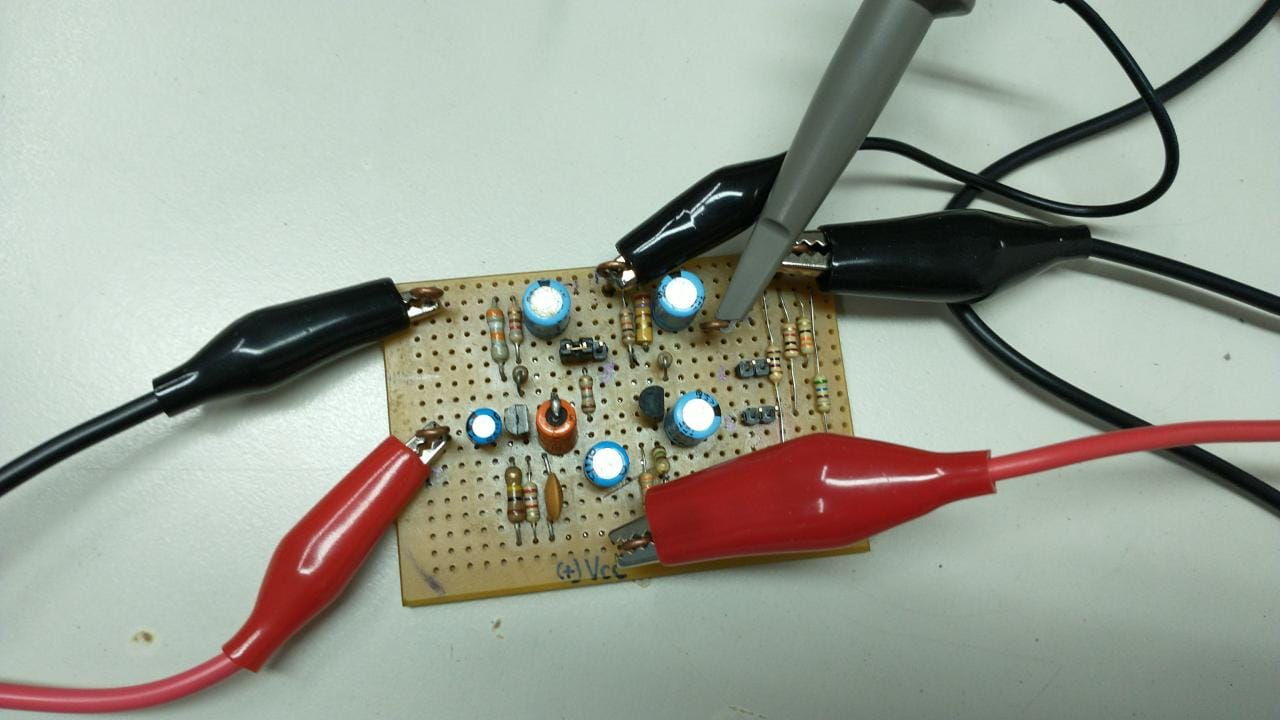
\includegraphics[width=0.8\textwidth]{Imagenes/ActividadPractica/7AnalisisDeDistorisonArmonicaEnAmpli/Amplificador.jpeg}}
          \caption{Amplificador a utilizar.}
          \label{fig:Exp7Amplificador}
        \end{subfigure}
        \hfill 
        \begin{subfigure}[H]{0.48\textwidth}
          \frame{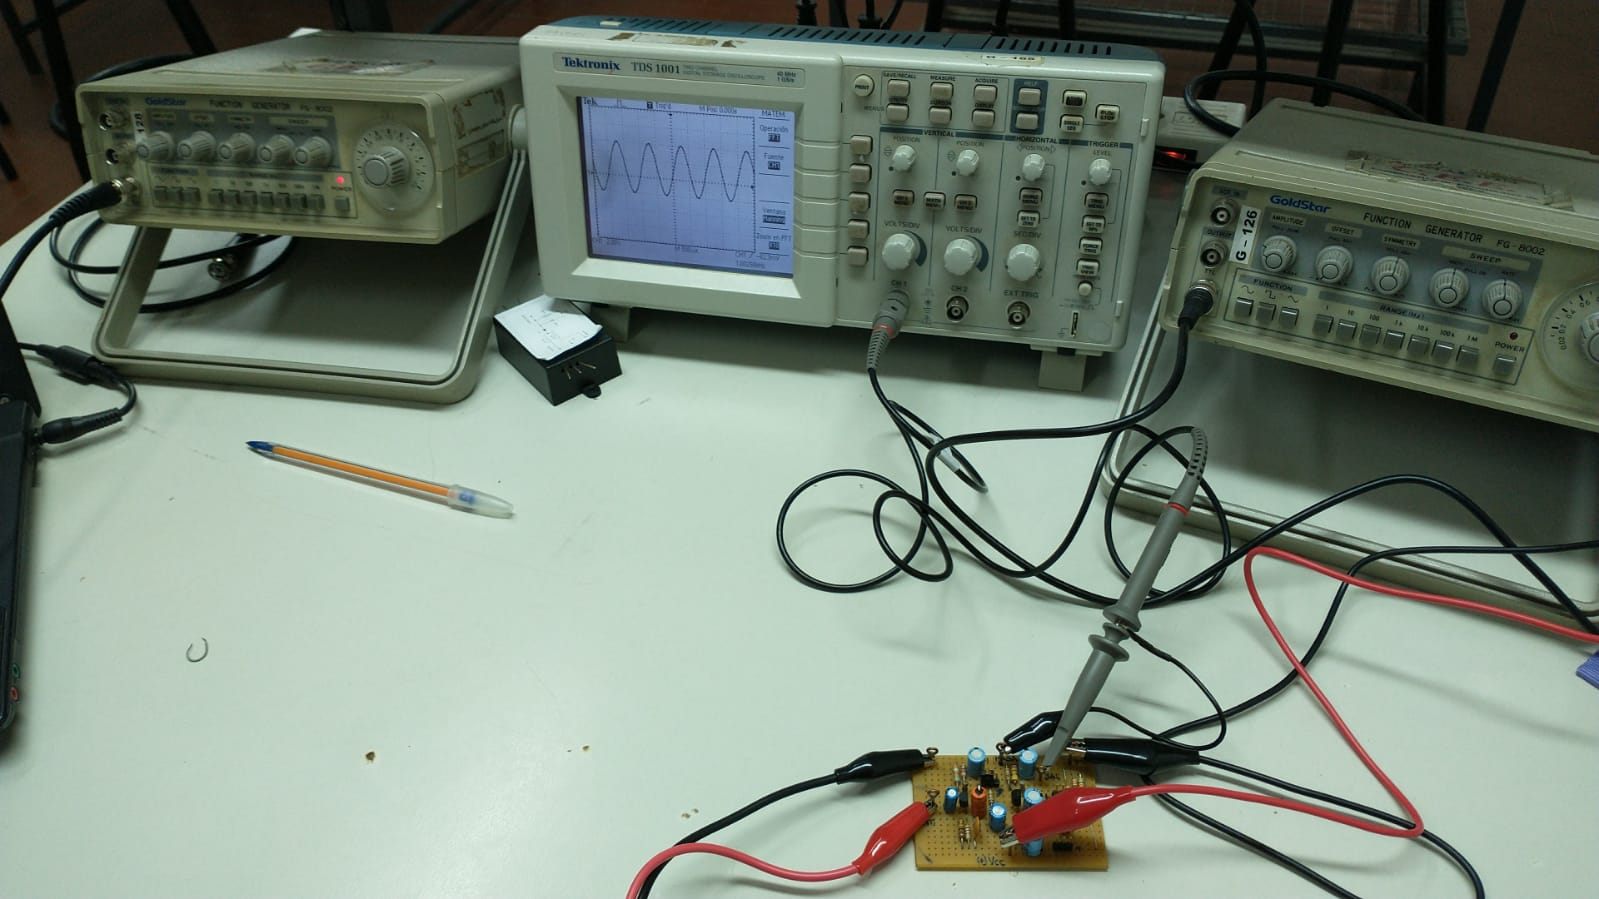
\includegraphics[width=0.8\textwidth]{Imagenes/ActividadPractica/7AnalisisDeDistorisonArmonicaEnAmpli/Equipo.jpeg}}
          \caption{Instrumental a utilizar.}
          \label{fig:Exp7Instrumental}
        \end{subfigure} 

          \caption{Amplificador a utilizar.}
          \label{fig:Exp7Circuito}
      \end{figure} 

    Inicialmente se configura para MES.

      \begin{figure}[H]
        \centering
          \frame{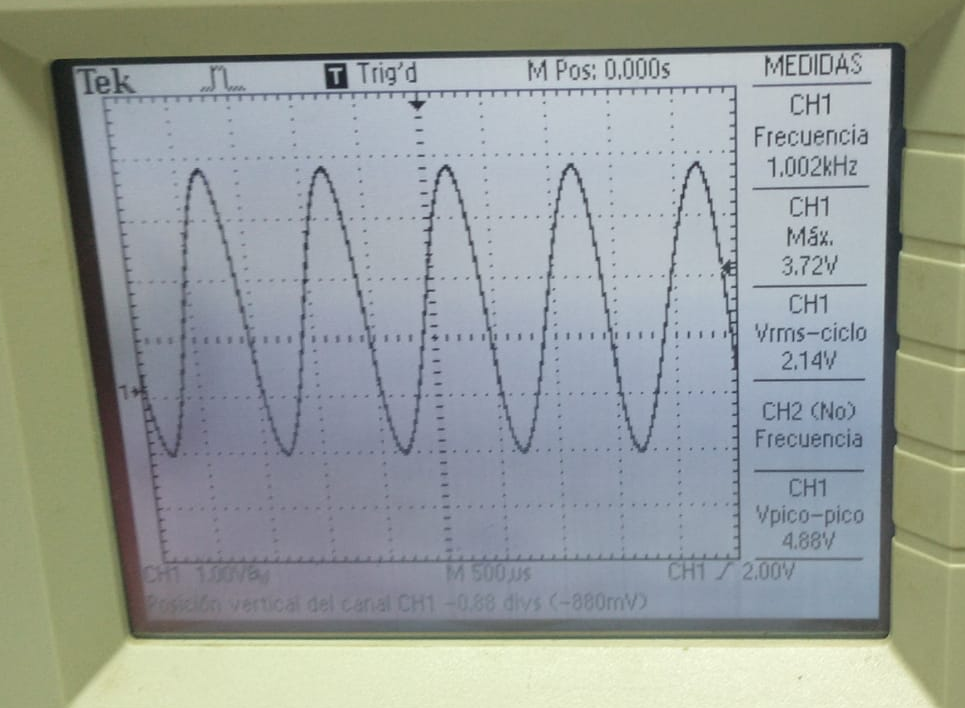
\includegraphics[width=0.8\textwidth]{Imagenes/ActividadPractica/7AnalisisDeDistorisonArmonicaEnAmpli/Exp7_MESlazoAbierto.png}}
          \caption{Máxima excursión simétrica a lazo abierto.}
          \label{fig:Exp7MESLazoAbierto}
      \end{figure}

      Luego se muestra la fundamental y sus dos primeros armónicos.

      \begin{figure}[H]
        \centering
        \begin{subfigure}[H]{0.48\textwidth}
          \frame{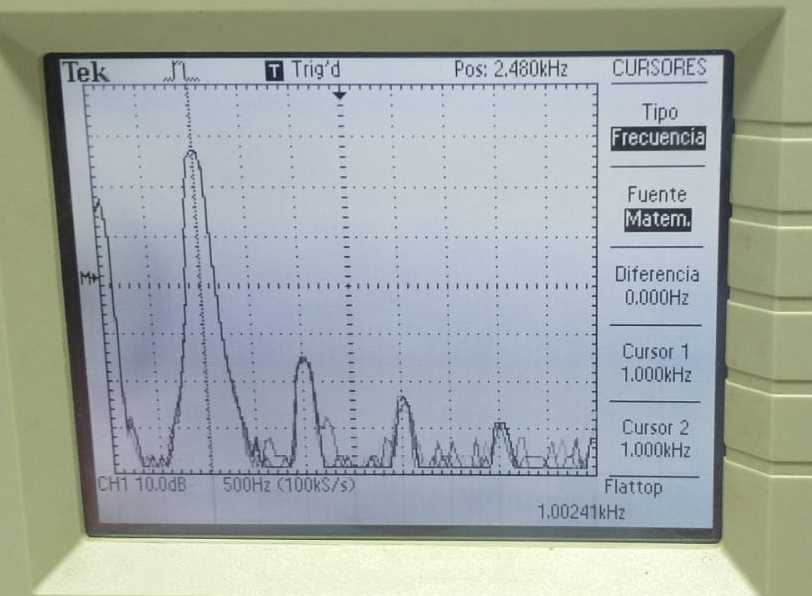
\includegraphics[width=\textwidth]{Imagenes/ActividadPractica/7AnalisisDeDistorisonArmonicaEnAmpli/Exp7_EspectroLazoAbiertoConCursorEn1k.png}}
          \caption{Frecuencia de la fundamental $f_{fund}=1~kHz$.}
          \label{fig:Exp7FrecFundamental}
        \end{subfigure}
        \hfill 
        \begin{subfigure}[H]{0.48\textwidth}
          \frame{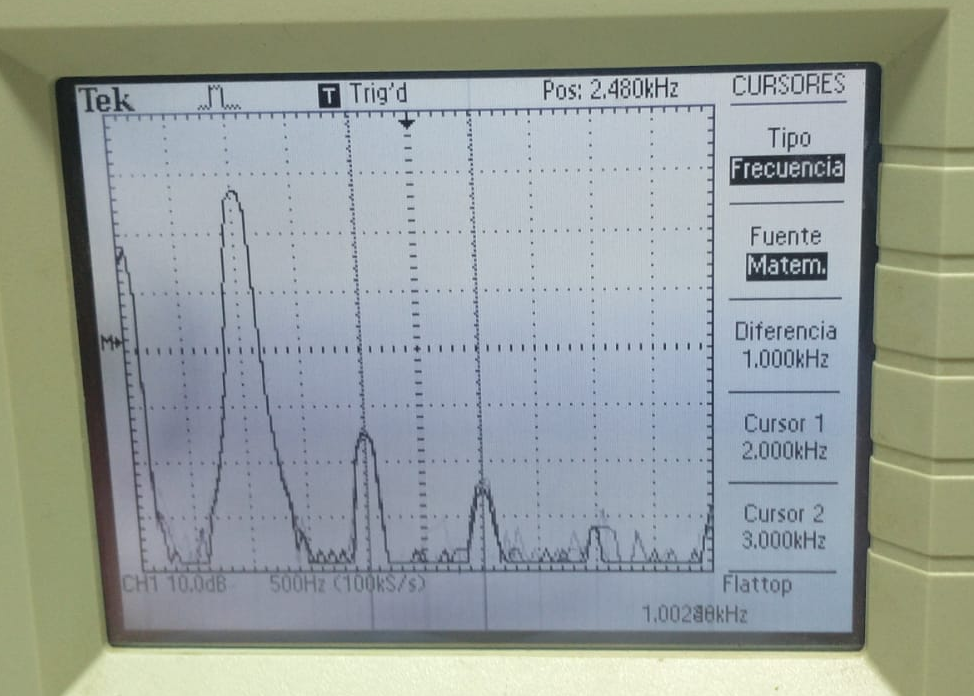
\includegraphics[width=\textwidth]{Imagenes/ActividadPractica/7AnalisisDeDistorisonArmonicaEnAmpli/Exp7_FrecuenciasDeLaSegundaYTercerArmonica.png}}
          \caption{Frecuencias de la segunda y tercer armónica $f_{2}=2~kHz$ y $f_{3}=3~kHz$.}
          \label{fig:Exp7Frec2da3raArmo}
        \end{subfigure}     
        \caption{Análisis espectral del amplificador con señal de $1~kHz$.}
        \label{fig:Exp7FrecFundYArmonicas}
      \end{figure}

      Luego se miden las amplitudes de la fundamental y armónicos.

    \begin{figure}[H]
        \centering
        \begin{subfigure}[H]{0.48\textwidth}
          \frame{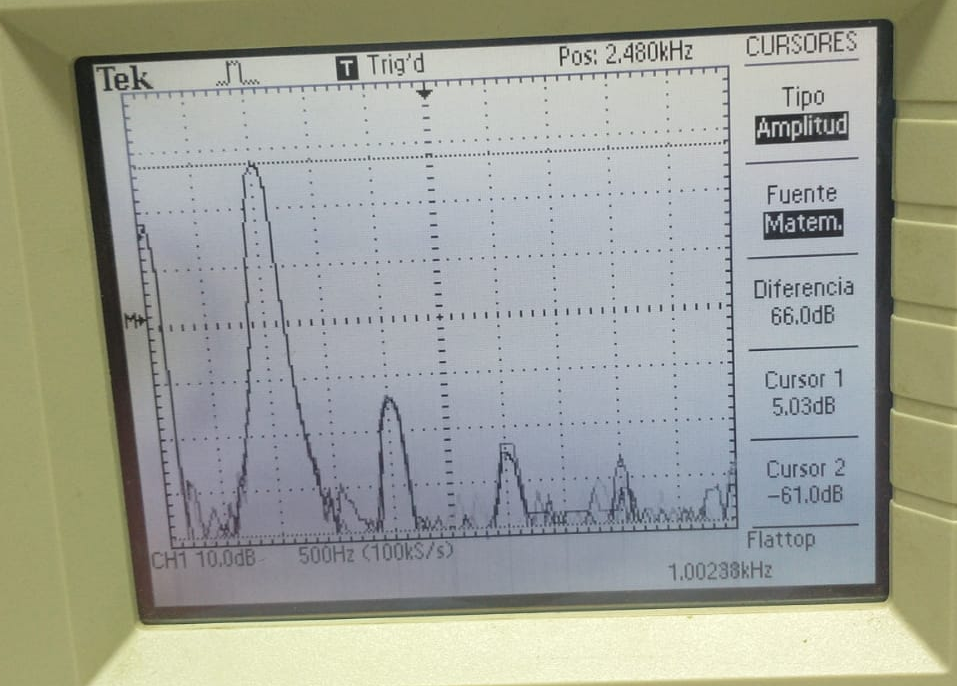
\includegraphics[width=\textwidth]{Imagenes/ActividadPractica/7AnalisisDeDistorisonArmonicaEnAmpli/Exp7_AmplitudDeLaFundamental.png}}
          \caption{Amplitud de la fundamental $V_{fund}=66~dBv$.}
          \label{fig:Exp7AmpFundamentalLA}
        \end{subfigure}
        \hfill 
        \begin{subfigure}[H]{0.48\textwidth}
          \frame{\includegraphics[width=\textwidth]{Imagenes/ActividadPractica/7AnalisisDeDistorisonArmonicaEnAmpli/Exp7_AmplitudDelSegundoArmónico.png}}
          \caption{Amplitud de la segunda armónica $V_{2da}=23,6~dBv$.}
          \label{fig:Exp7AmpSegundaLA}
        \end{subfigure}     
        \begin{subfigure}[H]{0.48\textwidth}
          \frame{\includegraphics[width=\textwidth]{Imagenes/ActividadPractica/7AnalisisDeDistorisonArmonicaEnAmpli/Exp7_AmplitudDelTercerArmónicoALazoAbierto.png}}
          \caption{Amplitud de la tercer armónica $V_{2da}=14~dBv$.}
          \label{fig:Exp7AmpTercerLA}
        \end{subfigure}   
        \caption{Amplitud de la fundamental y sus dos primeras armónicas.}
        \label{fig:Exp7AmplFundYArmonicasLA}
      \end{figure}

      Se repite el procedimiento, con la misma señal pero cerrando el lazo.

      \begin{figure}[H]
        \centering
          \frame{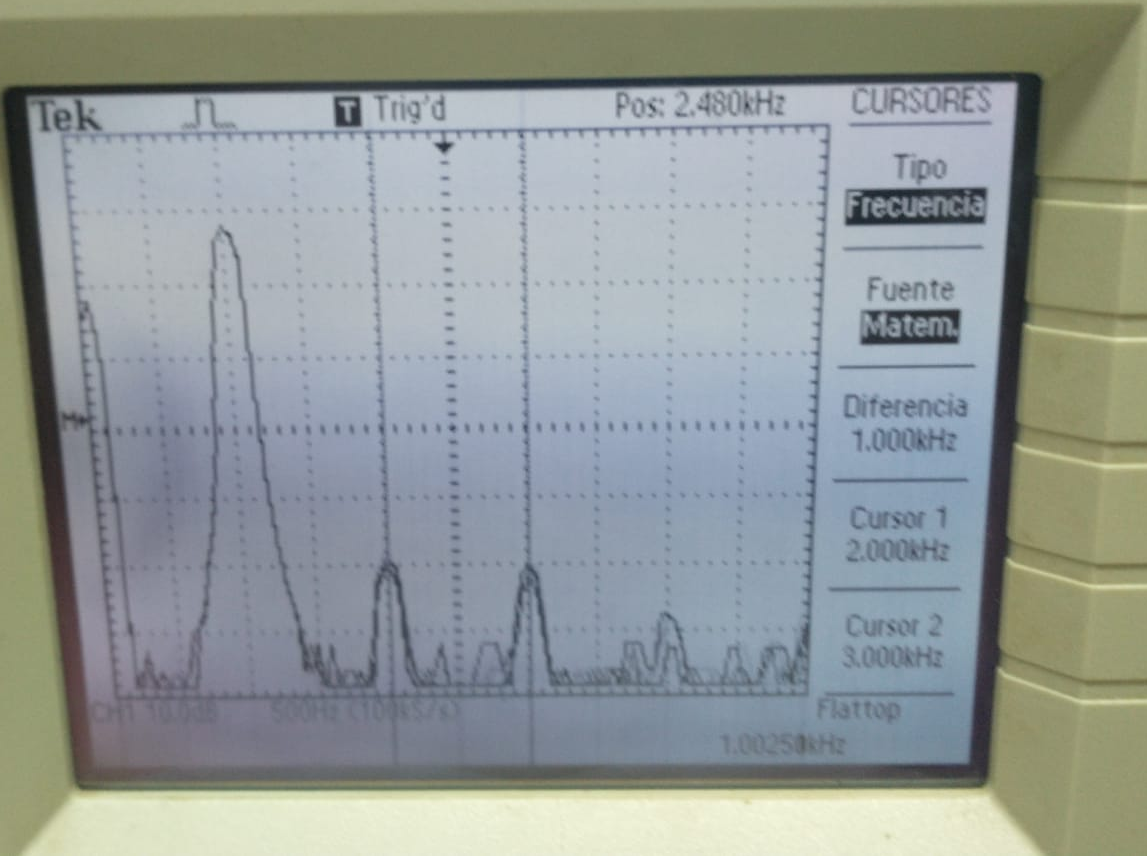
\includegraphics[width=0.8\textwidth]{Imagenes/ActividadPractica/7AnalisisDeDistorisonArmonicaEnAmpli/Exp7_LazoCerradoFrecuenciasDeSegundoYTercerArmonico.png}}
          \caption{Frecuencia de armónicos a lazo cerrado.}
          \label{fig:Exp7FrecLazoCerrado}
      \end{figure}

      Se mide la amplitud de los mismos.

      \begin{figure}[H]
        \centering
        \begin{subfigure}[H]{0.48\textwidth}
          \frame{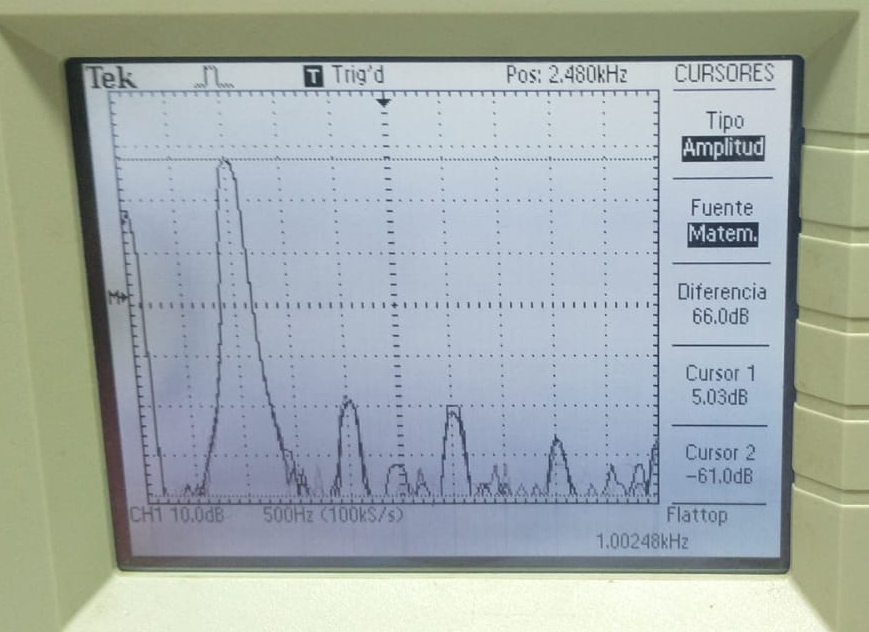
\includegraphics[width=\textwidth]{Imagenes/ActividadPractica/7AnalisisDeDistorisonArmonicaEnAmpli/Exp7_LazoCerradoAmplitudDelPrimerArmonico.png}}
          \caption{Amplitud de la fundamental $V_{fund}=66~dBv$.}
          \label{fig:Exp7AmpFundamentalLC}
        \end{subfigure}
        \hfill 
        \begin{subfigure}[H]{0.48\textwidth}
          \frame{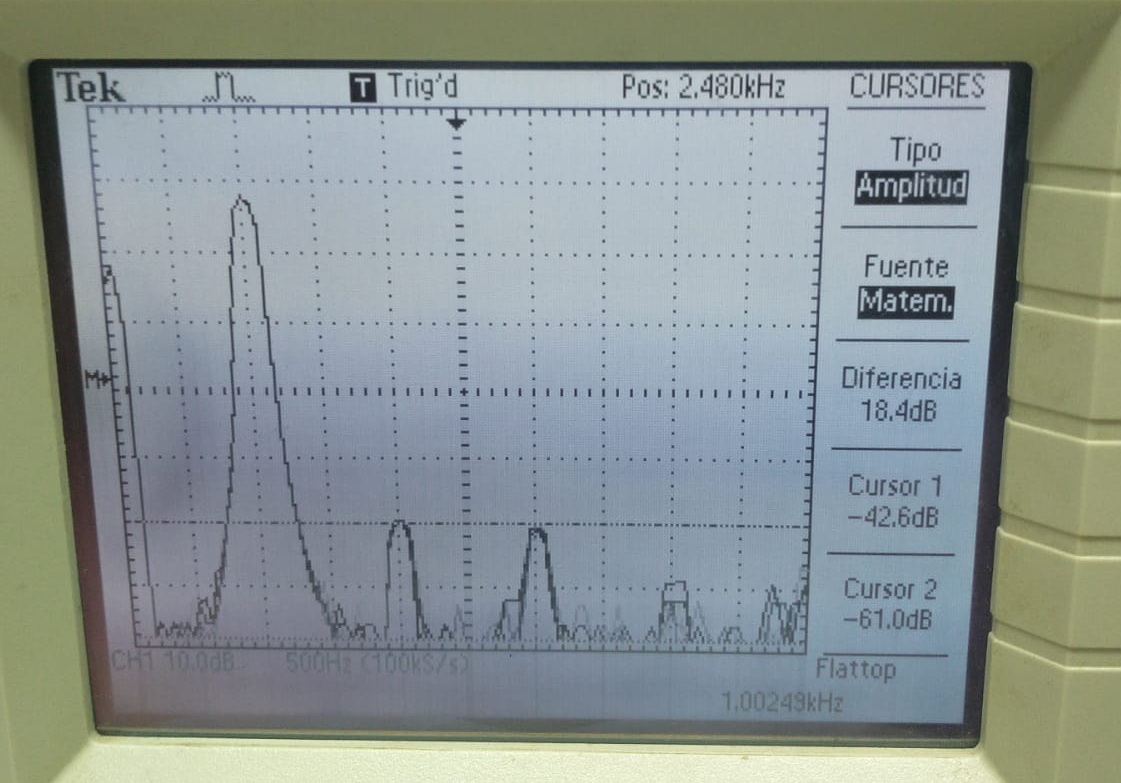
\includegraphics[width=\textwidth]{Imagenes/ActividadPractica/7AnalisisDeDistorisonArmonicaEnAmpli/Exp7_LazoCerradoAmplitudDelSegundoArmonico.png}}
          \caption{Amplitud de la segunda armónica $V_{2da}=18,4~dBv$.}
          \label{fig:Exp7AmpSegundaLC}
        \end{subfigure}     
        \begin{subfigure}[H]{0.48\textwidth}
          \frame{\includegraphics[width=\textwidth]{Imagenes/ActividadPractica/7AnalisisDeDistorisonArmonicaEnAmpli/Exp7_LazoCerradoAmplitudDelTercerArmónico.png}}
          \caption{Amplitud de la tercer armónica $V_{2da}=16,4~dBv$.}
          \label{fig:Exp7AmpTercerLC}
        \end{subfigure}   
        \caption{Amplitud de la fundamental y sus dos primeras armónicas.}
        \label{fig:Exp7AmplFundYArmonicasLC}
      \end{figure}    
      


